% Editable report section: Testing and Validation
\clearpage
\section{Testing and Validation}
\label{sec:5}

The current suite passed all 171 tests on Windows with Python 3.14.7. The JUnit record is \path{data/current-tests.xml}. Its 16.62-second runtime includes validation and interface work, so it is separate from construction timing. Fixed seeds and retained inputs make the cases reproducible.

\begin{table}[!htbp]
\centering
\caption{Current automated validation results: 171 passing tests.}
\label{tab:4}
\begin{tabularx}{\linewidth}{@{}Xrc@{}}
\toprule
\textbf{Test family} & \textbf{Cases} & \textbf{Result} \\
\midrule
Geometry, singular limits and AVL structure & 18 & Pass \\
Queue and circle events & 4 & Pass \\
Random, degenerate, scale and invalid inputs & 42 & Pass \\
Tight clusters and high degree & 14 & Pass \\
Parser, exports, CLI and callbacks & 4 & Pass \\
Pi regression cases & 4 & Pass \\
Replay model, Canvas and Matplotlib inspector & 53 & Pass \\
Precision frame and close-event regressions & 12 & Pass \\
Delaunay overlay and interactive bounds & 11 & Pass \\
Independent reference comparison tests & 9 & Pass \\
\bottomrule
\end{tabularx}
\end{table}

Ownership validation first locates queries in the generated polygons and then compares their assigned sites with an independent linear nearest-site scan. Empty-circle checks compare defining-site distances and scan all sites for an interior point; clipping corners are excluded because they need not be circle centres. The precision regressions also use exact input-circle identities to check empty circles without a distance tolerance. Area totals and per-site positive-cell assertions complement the sampled queries.

The current stress check passed 300 seeded configurations of 10--89 sites and forty tight-cluster configurations. Separate 100-, 1,000- and 10,000-site cases each checked 100 ownership queries and every emitted vertex, including all 19,978 vertices in the largest case. The expanded precision campaign passed 800 deterministic uniform, jittered-grid, clustered and ring configurations, using 100 ownership queries per configuration. Their records are \path{data/current-stress.json} and \path{data/precision-validation.json}.

\clearpage
\subsection{Independent Reference Comparison}

The validation-only comparator uses SciPy 1.18.1 for Voronoi ridges and Delaunay triangles \cite{scipyvoronoi,scipydelaunay}. SciPy is pinned in \path{requirements-reference.txt} and is absent from the construction imports. A separate Sutherland--Hodgman clipper constructs reference cells against every site using exact rational inequalities. It shares neither the production sweep nor its angle-sorted half-plane intersection.

The default comparison covers 30 random seeds, three transformed datasets and twelve minimal, degenerate, duplicate or near-coincident inputs. Every case checks clipped-cell boundaries and areas against the exact validator, and sampled ownership against a SciPy nearest-neighbour query. For general-position cases, the Delaunay edge sets are also compared. Cocircular inputs may have different valid triangulation diagonals.

All 45 cases passed the geometric checks. SciPy fully resolved 39 cases. Five minimal or collinear inputs are outside its two-dimensional construction, and one near-cluster case loses a site under Qhull's precision handling. The exact validator covers those six cases; they are recorded separately rather than counted as SciPy matches. No input perturbation is used to turn them into reference successes.

For box span $s$ and maximum coordinate spacing $u$, boundary comparison uses $2\times10^{-8}s+16u$, and cell-area comparison uses $2\times10^{-8}s^2+32us$. The JSON record retains each input, seed, box, tolerance, library version, discrepancy list and reference limitation. An intentionally corrupted overlapping cell is detected by the comparator's own regression test. These checks support the tested cases within the stated tolerances, rather than certifying every floating-point configuration.

The complete result and its reproducible inputs are retained in \path{data/reference-comparison.json}.

\clearpage
\subsection{Degenerate Cases and Numerical Stress}

\begin{center}
\begin{minipage}{\linewidth}
\captionsetup{hypcap=false}
\centering
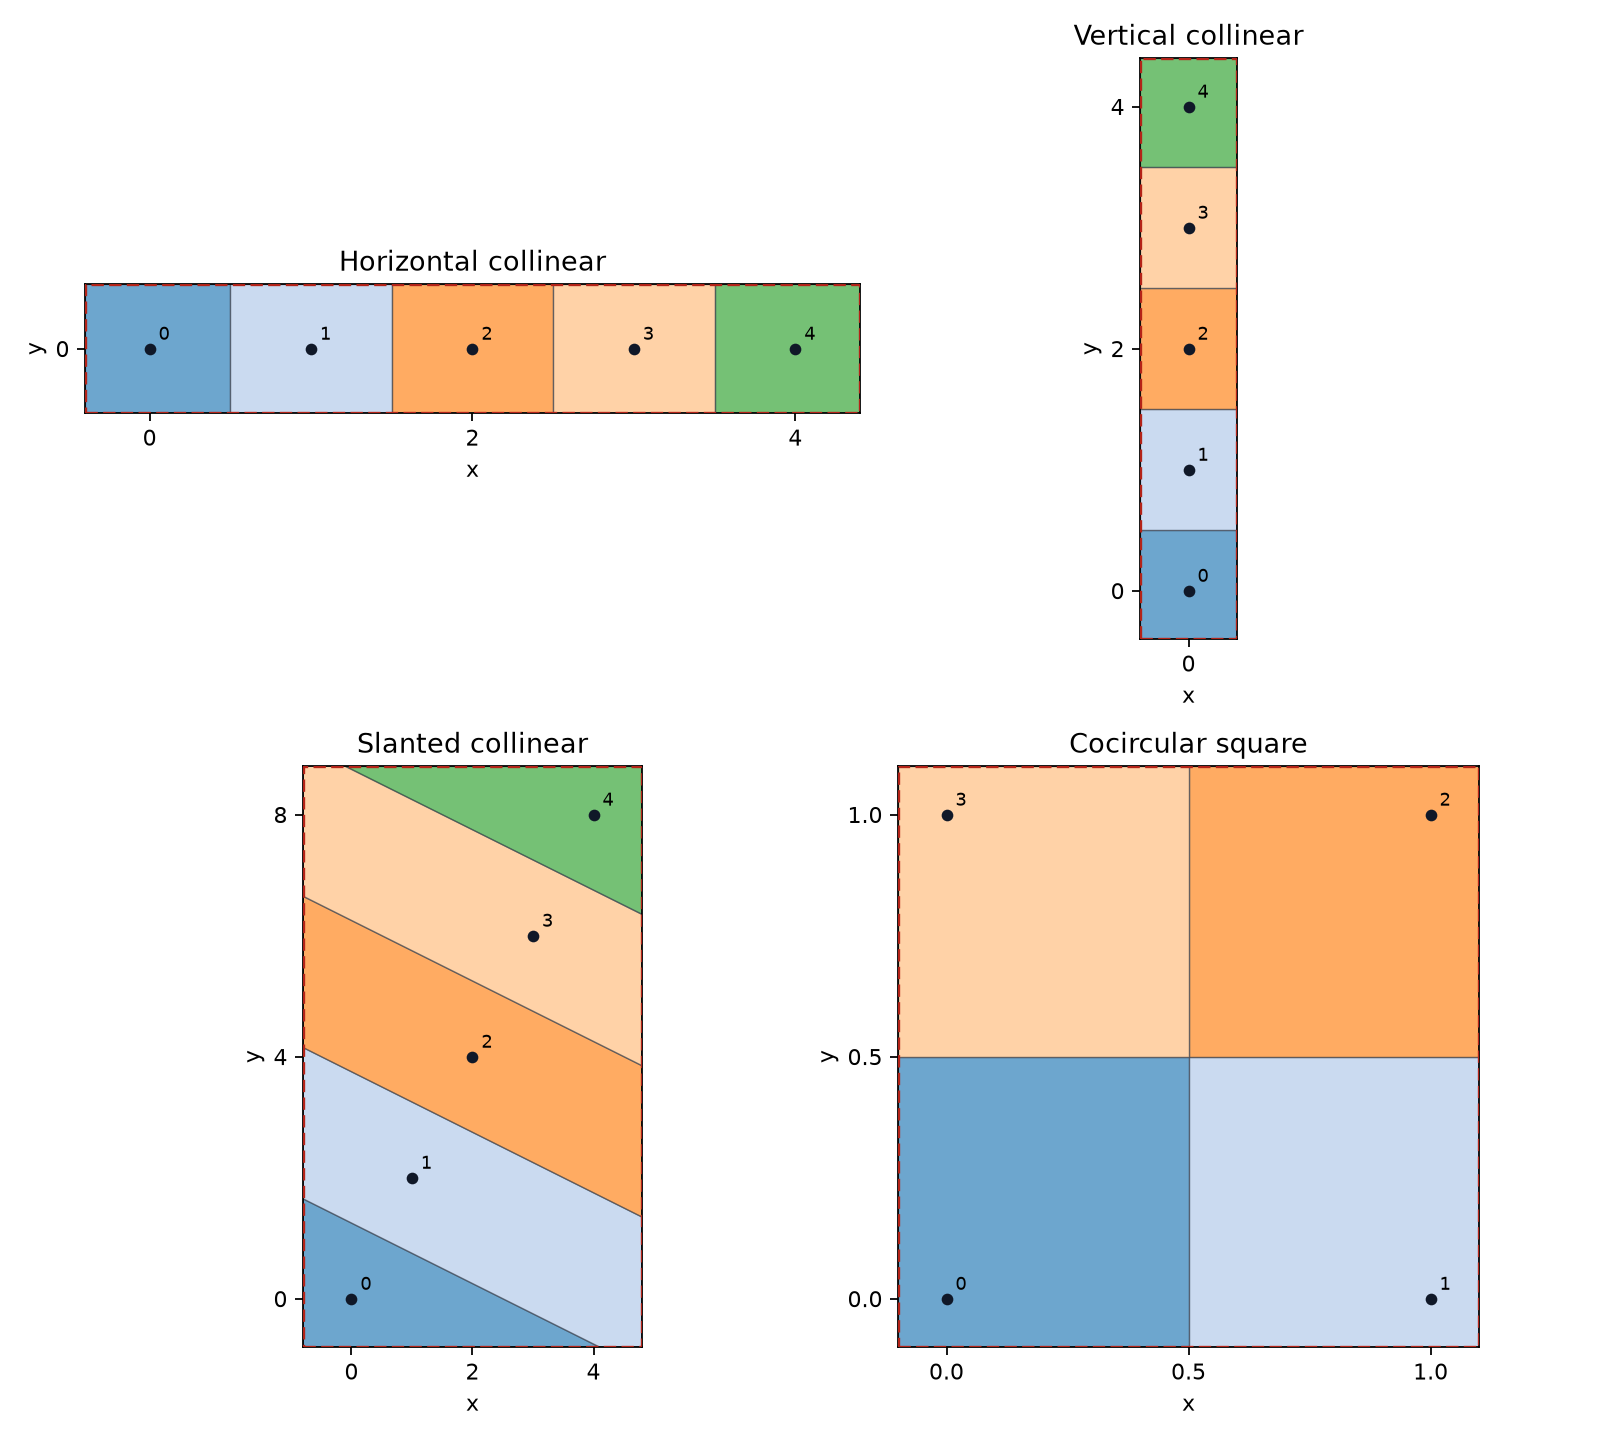
\includegraphics[width=1.0\linewidth,height=0.65\textheight,keepaspectratio]{degenerate-1.png}
\captionof{figure}{Horizontal, vertical and slanted collinear inputs, and a cocircular square.}
\label{fig:5}
\end{minipage}
\end{center}

The three line directions give parallel bisector strips. The square produces one common circle vertex; a zero-length diagonal is not drawn as a real edge.

\clearpage
\subsection{Duplicate, Nearly Coincident and Minimal Inputs}

\begin{center}
\begin{minipage}{\linewidth}
\captionsetup{hypcap=false}
\centering
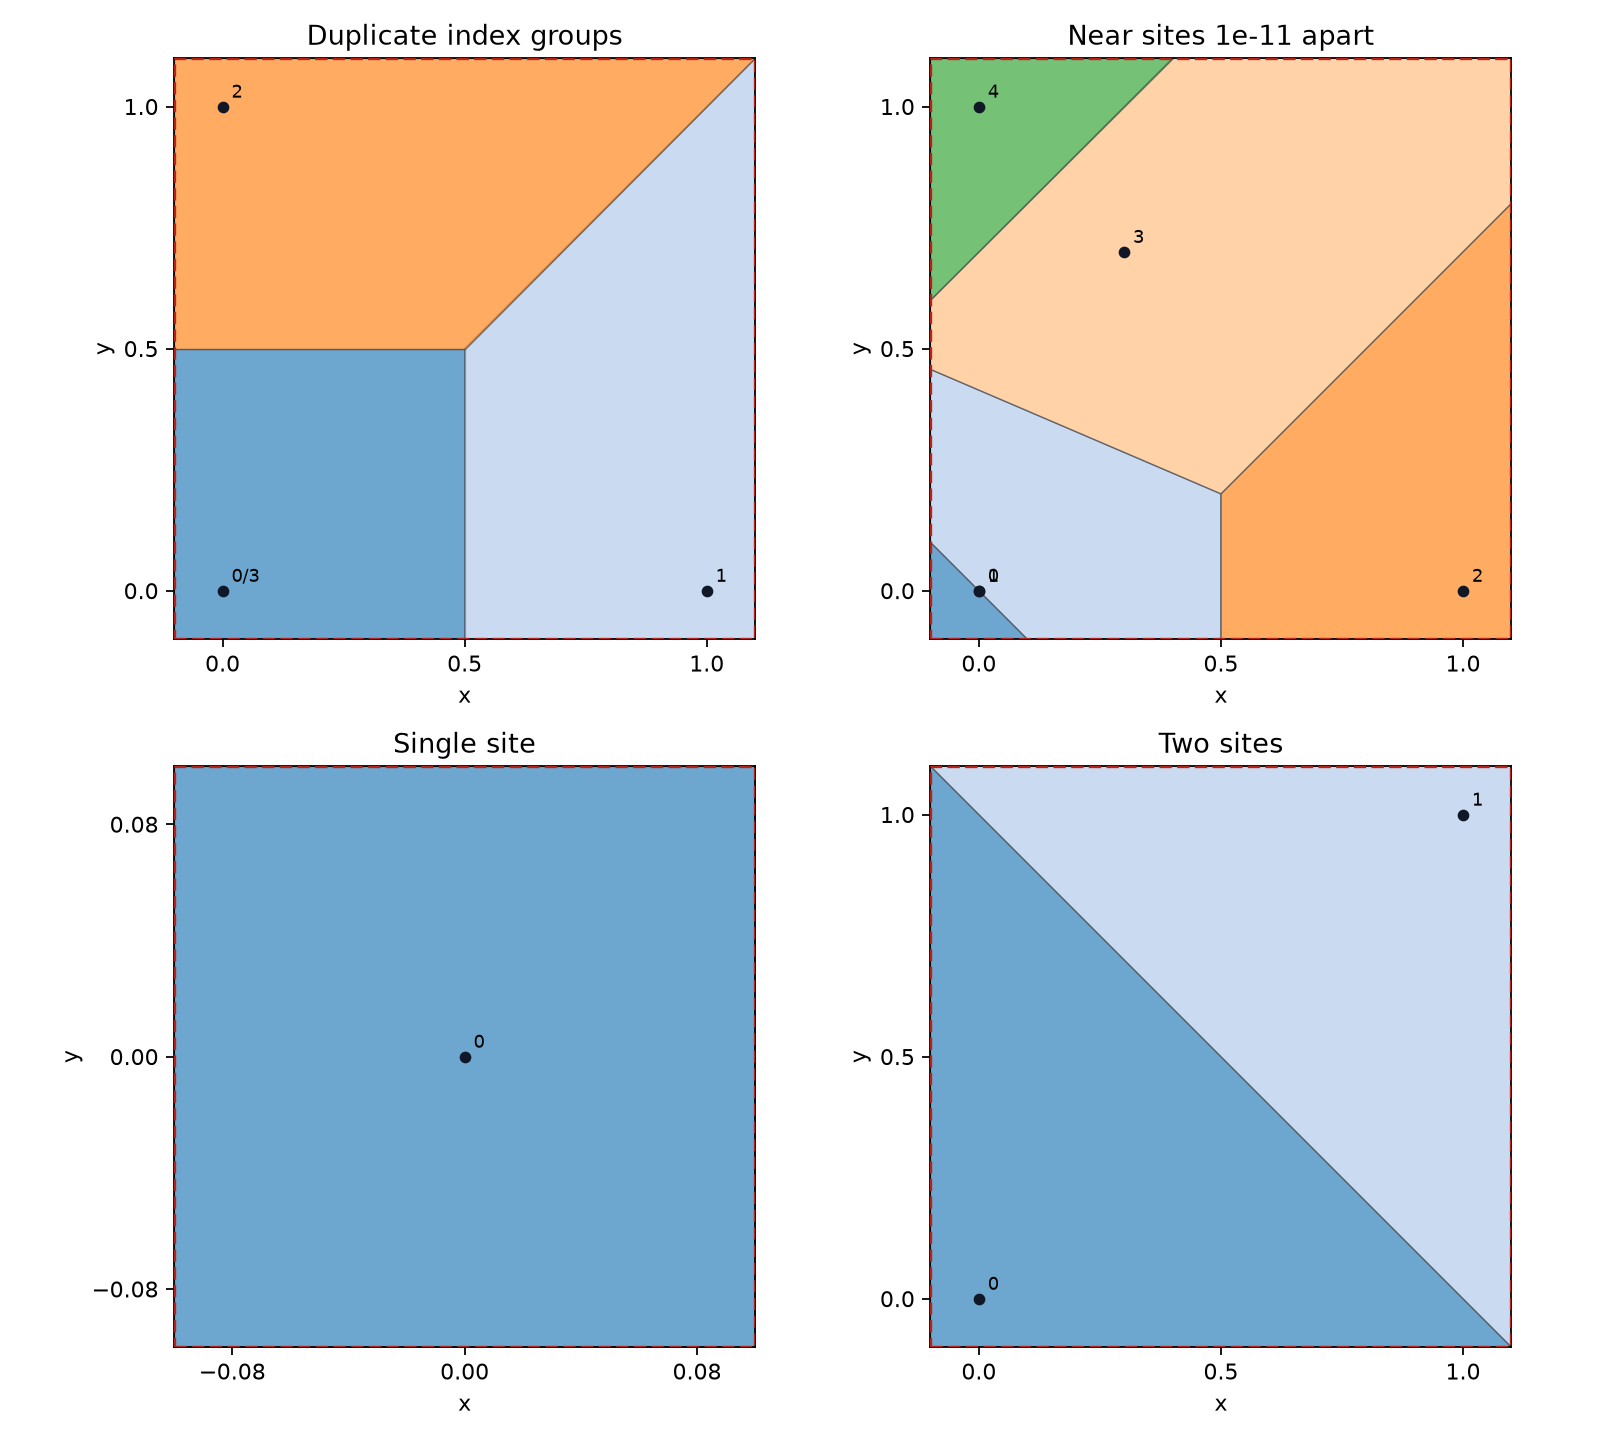
\includegraphics[width=1.0\linewidth,height=0.65\textheight,keepaspectratio]{degenerate-2.png}
\captionof{figure}{Duplicate, nearly coincident, single-site and two-site inputs.}
\label{fig:6}
\end{minipage}
\end{center}

Indices \code{0/3} in the duplicate example share one cell. In the near-site panel, sites separated by $10^{-11}$ are distinct but cannot be visually resolved at the full plot scale. Automated checks, rather than marker separation, establish their treatment. The adversarial tests additionally place six sites within clusters down to $10^{-15}$ among distant sites. Passing these cases under stated tolerances does not certify every near-degenerate input.


The numerical checks use tolerances that account for both construction error and the spacing of exported world coordinates. Passing a selected tight-cluster input therefore supports that case within its stated tolerances; it does not establish correctness for every possible floating-point input. Exact duplicates are grouped deliberately. The constructor rejects a coordinate range if its normalization loses subnormal bits.
